\documentclass[12pt]{article}

% Modernize grandpa Latex
\usepackage[utf8]{inputenc}
\usepackage[T1]{fontenc}
\usepackage{lmodern}

\usepackage[margin=1in]{geometry} % LaTeX wastes much space
\setlength{\parindent}{0pt} % Sets indent to zero

\usepackage{amsmath,amsfonts,amssymb,amsthm} % math tools and stuff
\usepackage{mathtools} % many detail improvements over ams and core tex

% write short pseudocode
\usepackage{verbatim}
\usepackage[ruled,vlined,linesnumbered]{algorithm2e}
\DontPrintSemicolon
\SetKwInOut{Input}{Input}
\SetKwInOut{Output}{Output}

\usepackage{graphicx} % required for images
\usepackage[shortlabels]{enumitem} % customizing enumerations
\usepackage{tikz} % helps drawing trees
\usepackage{xurl} % long urls to stay within the margin
\usepackage{forest} % simple trees
\usepackage{booktabs} % tables
\usepackage{float} % tables

% allows links, urls, and many other PDF tricks. 
\usepackage[
	pdftitle={PDFTITLEREPLACE},
	hidelinks,
]{hyperref}

\title{CS 247 Final Report}
\author{Roger Chen, Norman Chen, Peter Wang}
\date{}

%%%%%%%%%%%%% End of Preamble %%%%%%%%%%%%%

\begin{document}

\maketitle


\section*{Overview}

The project has 3 primary classes:
\begin{itemize}
	\item\textbf{Chess:} This is the main class 
	component of the project, responsible for 
	managing the overarching interactions of 
	the system. This is what gets instantiated 
	in the main function.
	\item\textbf{Game:} This manages a single 
	game state and encapsulates the core game
	logic and interactions.
	\item\textbf{Board:} This represents
	a single board state and encapsulates
	the logic for things like piece placement
	and movement.
\end{itemize}

The main relationships between these are that
\textbf{Chess Owns Games}. Chess can own as
many games as it wants because you can
play multiple games in a session. The
other main relationship here is \textbf{Game Owns
a Board}. This makes sense as each game is played on
one board, so each game object only owns a 
single board object. 

\bigskip

Each time the \textit{game} command is ran to play a new game,
the chess object will instantiate a new game object
for the game, and the game object will instantiate 
a new board object.

\bigskip

The \textbf{Chess} class also has a \textbf{owns a}
relationship with 2 other classes:
\begin{itemize}
	\item\textbf{DisplayBoard:} An abstract class with 
	\textbf{TextDisplay} and \textbf{GraphicsDisplay} as subclasses. 
	Responsible for displaying a text-based board and graphical board 
	(via X11) respectively to the user.
	An observer design pattern is deployed here.

	\item\textbf{Player:} Another abstract class with
	\textbf{Human} and \textit{\textbf{Computer}} as subclasses (Computer is abstract
	with concrete subclasses for each level). Responsible
	for facilitating moves from either a computer or
	human player.
\end{itemize}

\textbf{Chess} will typically own 2 \textbf{DisplayBoard}
objects, one for the console version and
one for the graphical version. When the chess object gets instantiated, the 
DisplayBoard objects are also instantiated. Both
displays are instantiated by default, but
the graphics display can be omitted via a
command line argument.


\bigskip

\textbf{Chess} can also own as many player 
objects as it since multiple games with different players
can be played in a single session. Whenever
a new game is created, the chess object
will instantiate 2 more player objects.
We store all the games and players
for possible future additions.

\bigskip


The \textbf{Board} class also
\textbf{owns \textit{Pieces}}. 
\textbf{\textit{Pieces}} is an abstract class with
a concrete subclass for each of the 6 types of pieces.
A board object can own as many piece objects
as a board can allow. When a board
object gets instantiated, the board
will instantiate the required number
of piece objects for the desired board.

\bigskip

When a \textit{move} command gets
ran, the command is first parsed
by the chess object. Then the chess
object calls the corresponding
$make\_move$ function for either
the human or computer player. This
function calls the game object
to validate and execute the move
with the board object.

\bigskip

At the same time, the chess
object notifies the displays to
display the board. The boards
get the state from the chess
object then displays the
new state.

\bigskip

We also have command line flags. These command line flags include

\begin{itemize}
	\item \textbf{--no-graphics} or \textbf{-ng}: This flag disables the graphical interface, for development in environments that do not support X11.
        \item \textbf{--no-strict} or \textbf{-ns}: This flag disables strict mode for input. Strict mode throws errors when invalid inputs / arguments are given. Non-strict mode catches these errors and allows for the user to re-enter inputs.
\end{itemize}


\section*{Updated UML Diagram}
The updated UML diagram is highlighted below:
\begin{figure}[H]
	\centering
	\includegraphics[width=0.8\textwidth]{uml.png}
	\label{}
\end{figure}


Throughout the development process, 
we had to make adjustments to our 
initial UML diagram in order to make 
everything work together.

\subsubsection*{Display Ownership}
The main difference between the updated and initial UML diagram was that we moved the ownership to the displays (both graphical and text based) from the \textit{Game} object to the \textit{Chess} object. This allowed us to have one display for each chess instance, instead of heaving to maintain a vector of displays for each Game.

\subsubsection*{Additional Helper Methods \& Fields}
There were also many helper methods and additional fields that we had to include in our program beyond our initial considerations. For example, boolean fields had to be maintained to track whether en-passant or castling was optional for each player.

\subsubsection*{Global Structures}
We discovered that maintaining global structures, such as \textit{PieceTypes} and \textit{Color}, throughout the program was significantly easier. This approach contrasted with our initial method of embedding these structures within classes, which required additional code and complexity.


\section*{Design}

\subsubsection*{Smart Pointers}

We helped solve the problem of memory management
through vectors and smart pointers. For example,
the ownership of our display classes 
were represented via unique pointers in our
chess class. The games and players
were also represented with a vector 
of smart pointers in the chess class.
Moreover, "has-a" relationships between objects
were represented via weak pointers.

\bigskip

Because of this, we were able to not 
explicitly managing our own memory and have
no delete statements, making development easier
to and simply without worrying as much with memory.

\subsubsection*{Dynamic Casting}

We use dynamic casting to help with en-passant
and castling. In castling, we need to check
if the king is in check in order to be
able to castle. Dynamic casting helps
us achieve this since we can dynamic
cast the piece in the board class method
to king in order to call its $in\_check$ function.

\bigskip

Likewise, dynamic casting has helped us
with en passant. It helps us call 
the $get\_valid\_moves$ method in Pawn
in order to help us determine
whether we can en passant. Dynamic
casting has helped simplify and improve 
our code by improving cohesion, since each
concrete piece class tries to handle
its own logic for specific chess rules.

\subsubsection*{Observer Pattern}

For the graphics part, we employed the observer
design pattern. The chess class is the concrete subject
and the DisplayBoard class is the abstract observer.
The concrete graphics and text display classes
are the concrete observers. 

\bigskip

This helps
improve cohesion as
the display observers only job is to display
the chess board it has. It also helps
reduce coupling as the display logic 
is not as tightly coupled to the chess class. Thus
the project is more maintainable and easier to work on.

\subsubsection*{Strategy Pattern}

The Player class employs the strategy design pattern,
particularly the computer and each of its levels. By
defining the player class as abstract and implementing 
each type of player as a concrete subclass, it is easy
to add in new strategies with new subclasses (like
new computer levels).

\bigskip

This also follows the open/close principle. For example, if you want
a new level for computer, you simply add a new subclass
to Computer instead of having to modify an 
entire Computer class or something in that nature if
the strategy pattern wasn't applied.

\subsubsection*{Template Pattern}

Our Piece class follows a template pattern.
The piece abstract class has the template method
$get\_threatened\_squares$. Each concrete
piece class implements this method in
its own way to help provide their specific
movement and capture logic. The piece class
just defines the overall structure of the piece
and provides common functionality.

\subsubsection*{Coupling and Cohesion}

During our design and implementation, we aimed
to minimize coupling and maximize cohesion. We
achieved these things by employing a variety of 
different design patterns and OOP principles. 

\bigskip

For example, our template pattern
helped with coupling by separating
the piece logic from the board itself, it
also helped with cohesion since each
piece is just responsible for the spaces
it can threaten. 

\bigskip

We also minimized coupling by having no friend
classes or global variables for game logic 
(we had global variables for debugging flags,
but none for game logic).

\bigskip

Cohesion was maximized by having many classes
for each part of the game. Splitting the core
game into the 3 classes (chess, game, and board), 
and having each piece, player, and display
as its own class really helped maximize cohesion
as each class has its own single clear objective.

\section*{Resilience to Change}

Given our high cohesion, any
specific changes to certain parts of the program
can be easily made by simply going to the class
and making the change there.

\bigskip

Furthermore, due to our low coupling, any changes in
our classes are unlikely to break anything else.
For example:

\subsubsection*{Simultaneous Games/Game History Support}

We store all the games and players that 
play in a vector. When a new game starts
we simply append to the game and players
vector in the chess class. Because of this,
if we wanted to support simultaneous games
we could add support for "pausing" games
and allow the user to go back in the vector
to play a past game. It also supports
game history a since you can
go back in the vector to look at
past game states and informatiom.

\subsubsection*{Undo Operation}

Our board has FEN support 
(a concise way to represent a chess board as a string).
We have a FEN serializer and deserializer and our
board has a constructor that takes in a FEN 
value to create the board. 

\bigskip

Because of this, we simply store the FEN
after each move in a string vector. 
To undo a certain number of moves we just
use the find the corresponding FEN value and recreate
the board with it with our serializer.


\subsubsection*{New Pieces/Piece Rule Changes}

Because we employ the template design pattern,
adding in new pieces is quite easy
as all you need to do is add a new subclass
to Piece and write the $get\_threatened\_squares$
function for the pieces behaviour.

\bigskip

If you want to change the behaviour of an existing
piece it is also quite simple, just go to the pieces
class and modify just the template method. Template
design makes this feature simple as typically only you
only need to focus on the one function.
\subsubsection*{New Computer Levels/New Players}
Again, because we implement the strategy
design pattern, adding in new computer levels
or any new player types is easy. All you would 
need to do is add a new subclass for the
player/level. 

\subsubsection*{Fun Game Modes}
We could implement game modes like, no Queen
or no pawns. Or even game modes where one player
is down certain material. We could implement
these via our setup function for creating
any board state and wrapping it around
the new command for the game mode.

\section*{Extra Credit Features}
\subsubsection*{Sophisticated Graphics Display}

Having visually appealing graphics was a challenge. 
The provided Xwindow class had very little
functionality builtin, so we had to learn a good
amount of X11 and heavily modify the 
Xwindow class to get clean graphics. We were able to import images of the actual chess pieces with color coding into our graphical display, as seen in the screenshot below.

\begin{figure}[H]
	\centering
	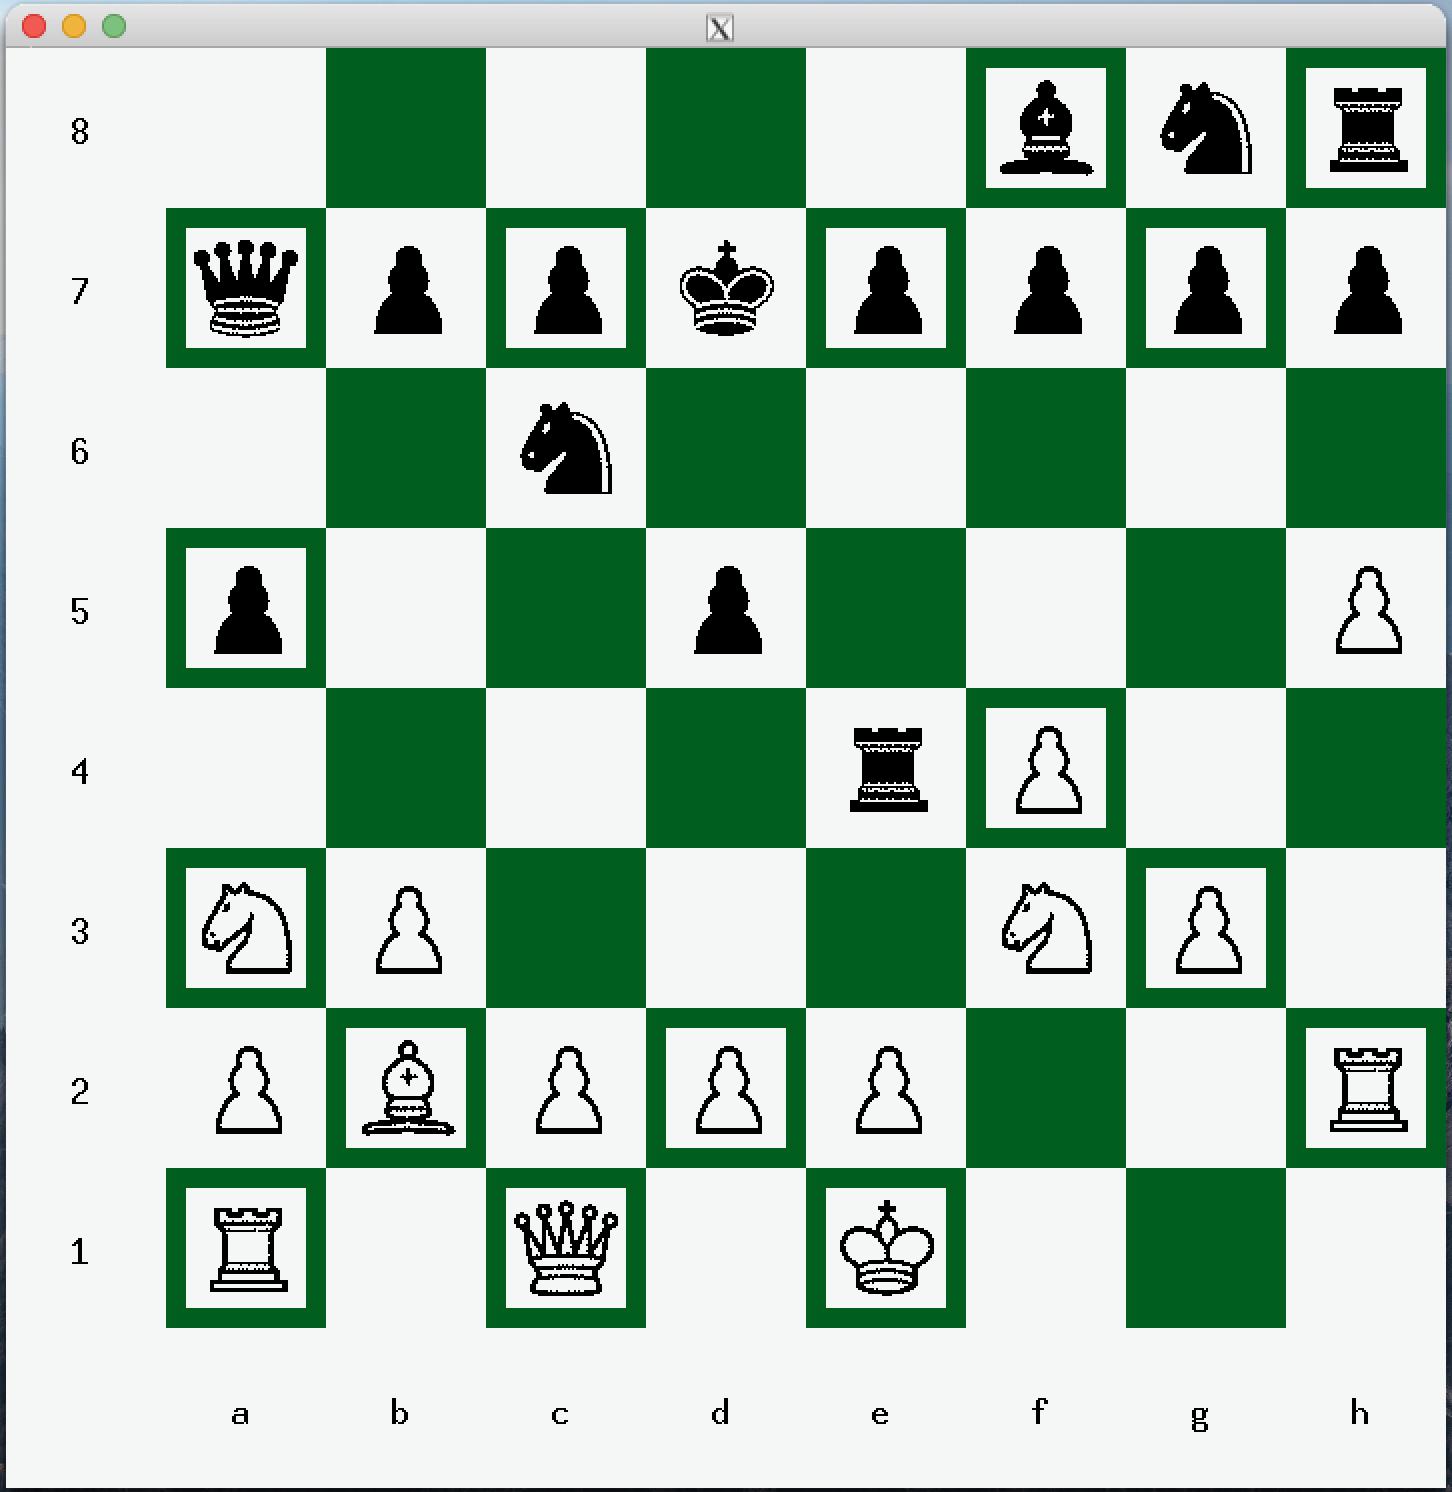
\includegraphics[width=0.5\textwidth]{graphic.png}
	\label{}
\end{figure}

For example, in order to use images, we had to get
bitmap of each image. This involved
converting the image of each individual chess piece
to a bitmap and importing it in. Then
we had to use the \underline{Pixmap functions}
of X11 to actually render it, this made the 
graphical display much more visually appealling to work with.

\subsubsection*{Comprehensive Test Suite}

A comprehensive test suite was generated by taking public
machine learning game data from Hugging Face's \href{https://huggingface.co/datasets/laion/strategic_game_chess?row=0}{\underline{chess dataset}}. These games are the result of Stockfish 16.1 playing itself. We took over 1000 games and parsed them into our own input and output format as test cases.

\bigskip

The test cases are in the \textit{.in} and \textit{.expect} format, which can be found under the 'tests/in' and 'tests/expect' directories respectively. 

\subsubsection*{Continuous Integration \& Continuous Development (CI/CD) Pipeline}
To ensure that additional features added to our chess program did not break basic functionalities, we implemented a modern CI/CD pipeline using \href{https://github.com/PeteMango/CS247-Chess/actions}{\underline{Github Actions}} with over 1000+ test cases as mentioned above. Correctness testing was conducted on every push and pull request, whereas the longer and more sophisticated memory tests with Valgrind was conducted every hour.

\subsubsection*{Level-5 Computer}

In addition to the already advanced level-4 computer, we implemented a level-5 computer program that consistently beat every other level (including level-4 with over 90\% checkmate rate) in less than 200 moves.

\bigskip

Additional features of the level-5 computer include:
\begin{itemize}
    \item \underline{Checkmate Detection}: Detecting and executing immediate checkmates (mate in one) if such a move exists, as this has the highest priority.
    \item \underline{Favorable Trades}: Engaging in trades only if they are favorable, meaning the piece taken is more valuable than the piece that could be lost on the next turn.
    \item \underline{Simultaneous Check/Capture/Escape}: Prioritizing moves that achieve multiple objectives, such as delivering a check, capturing a piece, and escaping from an attack, over moves that accomplish only one of these tasks.
    \item \underline{Capture Value}: Out of all possible captures, select the one with the highest value.
    \item \underline{Escape Value}: Among pieces under attack, move the most valuable piece out of danger.
    \item \underline{Endgame Strategy}: Prioritize checking rather than protecting pieces in the end game, as this would make it easier for checkmates to occur
\end{itemize}

\section*{Final Questions}
\subsubsection*{1. What lessons did this project teach you about developing software in teams? If you worked alone, what lessons did you learn about writing large programs?}
Building and developing this chess program provided many valuable lessons and takeaways for each team member.
\begin{itemize}
    \item \textbf{Division of Labor}: One of the most important aspects contributing to the success of our project was the equitable division of work among team members. By tracking each member’s progress and redistributing tasks as needed, we ensured that everyone contributed effectively and no one was overwhelmed by their workload.
    \item \textbf{Modular Design \& Documentation}: The modular design of our program facilitated smooth division of labor. Each member could work on different parts of the program independently, without waiting for others to finish their tasks. Detailed documentation and comments enabled team members to quickly understand each other’s work, ensuring seamless transitions between different stages of the project.
    \item \textbf{Importance of Version Control}: Our prior co-op experiences underscored the importance of version control systems like Git in team environments. We utilized branches to maintain a working version of our software, preventing conflicts during development. Additionally, Git allowed us to conduct effective code reviews, incorporating multiple opinions before merging changes into the main branch.
    \item \textbf{Test Driven Development (TDD)}: Focusing on TDD throughout our development process gave us confidence in our code changes. Writing tests before implementing features ensured that new additions did not break existing functionality, maintaining the integrity of the chess game.
    \item \textbf{Continuous Integration and Continuous Development (CI/CD)}: Early in the project, we set up a CI/CD pipeline using GitHub Actions. This automated the running of our test suite on every code push, pull request, and merge, ensuring that our changes did not break the production environment without manual intervention.
\end{itemize}
\subsubsection*{2. What would you have done differently if you had the chance to start over?}
If we had the opportunity to start from scratch, we would make some key changes:
\begin{itemize}
    \item \textbf{Improved Initial UML Diagram}: Spending more time on the initial UML diagram to ensure all cases are considered would have minimized design changes during coding. A comprehensive UML diagram would provide a holistic view of the project, preventing surprises during development.
    \item \textbf{Reduce Code Redundancy}: We would focus on reducing code redundancy. Many components shared similar functionalities but had separate functions. Consolidating these into single, more versatile functions would optimize the codebase and improve maintainability.
    \item \textbf{Integrated Test Suites}: We would integrate tests directly within our program using libraries such as GTest, instead of relying on external tests via shell or Python scripts. This integration would enable more sophisticated and detailed checks on valid moves, checkmates, and overall game logic for both human and computer players.
    \item \textbf{Performance Optimizations}: Focusing on performance optimizations, especially for the computer logic, would allow for faster computations and deeper searches of possible outcomes. This would enhance the efficiency and effectiveness of the chess engine, providing a more challenging and responsive experience.
\end{itemize}
\section*{Conclusion}
In conclusion, this project provided us with real world examples of C++ concepts and software engineering design principles. This experience also helped us develop crucial teamwork skills, which will be extremely crucial for our future careers. Overall, it was a fun project that we all enjoyed and had a fun time building.\end{document}